\documentclass[UTF8]{standalone}
\usepackage{tikz}
\usetikzlibrary{positioning}
\usepackage{ctex}

\begin{document}
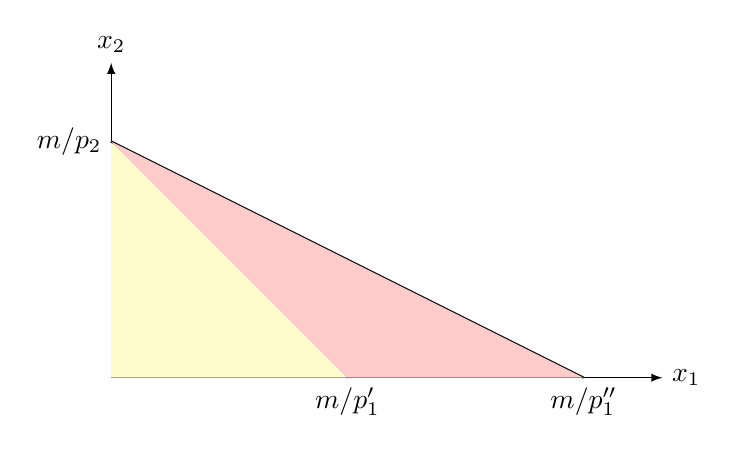
\begin{tikzpicture}
    \draw[-latex] (0,0) -- (7,0) node[right] {$x_1$};
    \draw[-latex] (0,0) -- (0,4) node[above] {$x_2$};

    \draw[domain=0:3, thick] plot (\x, {-\x+3});
    \node[left] at (0,3) {$m/p_2$};
    \node[below] at (3,0) {$m/p_1'$};

    % \node at (2,3) {$p_1x_1+p_2x_2=m$};

    \coordinate (A) at (0,0);
    \coordinate (B) at (3,0);
    \coordinate (C) at (0,3);
    \fill[yellow!20] (A) -- (B) -- (C) -- cycle;

    \draw[domain=0:6, thick] plot (\x, {-\x/2+3});
    \node[below] at (6,0) {$m/p_1''$};

    \coordinate (D) at (6,0);
    \fill[red!20] (B) -- (C) -- (D) -- cycle;
 
\end{tikzpicture}
\end{document}